\section{Experiments}
\label{sec:experiments}

\pgfplotsset{compat=1.17}

% --- Preamble: Define custom plot styles for statistics ---
\pgfplotsset{
    % Common style for all subplots in this figure
    stats multiplot style/.style={
        width=\linewidth,
        height=5.5cm,
        ybar,
        bar width=10pt,
        xtick=data,
        symbolic x coords={ERM, Median, Mean, SODA},
        xticklabel style={rotate=45, anchor=east, font=\small},
        ymajorgrids=true,
        grid style=dashed,
        enlarge x limits=0.15,
    },
    % Define the color for each bar class
    scatter/classes={
        ERM_class={fill=gray!60, draw=gray!80},
        median_class={fill=blue!30, draw=blue!70},
        mean_class={fill=blue!60, draw=blue!90},
        max_class={fill=purple!60, draw=purple!90},
        soda_class={fill=orange!80, draw=orange!90}
    }
}
\begin{figure*}[htbp]
    \centering
    
    % --- Single addplot with a table for each subplot ---
    
    \begin{subfigure}{0.32\textwidth}
        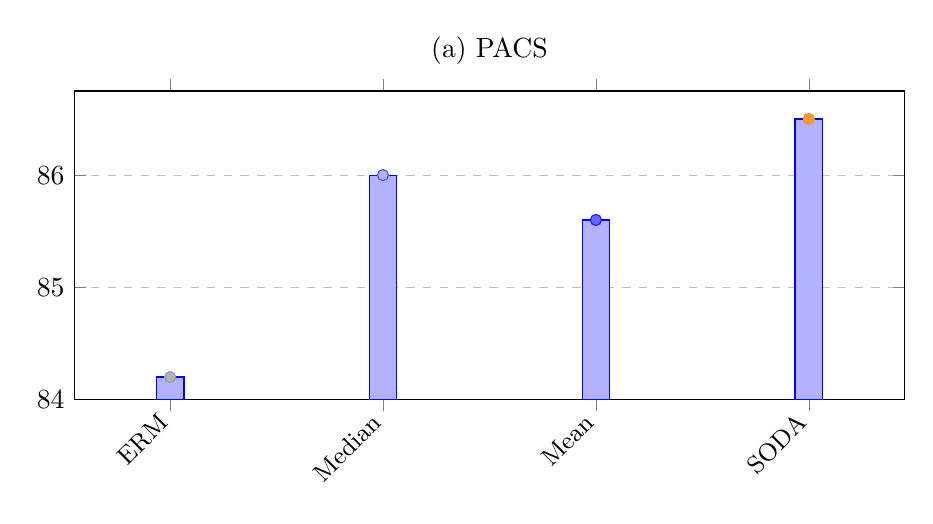
\begin{tikzpicture}
            \begin{axis}[stats multiplot style, title={(a) PACS}, ymin=84]
                \addplot+[scatter, scatter src=explicit symbolic] 
                table [meta=class, col sep=comma] {
                    x,      y,      class
                    ERM,    84.2,   ERM_class
                    Median, 86.0,   median_class
                    Mean,   85.6,   mean_class
                    SODA,   86.5,   soda_class
                };
            \end{axis}
        \end{tikzpicture}
    \end{subfigure}
    \hfill
    \begin{subfigure}{0.32\textwidth}
        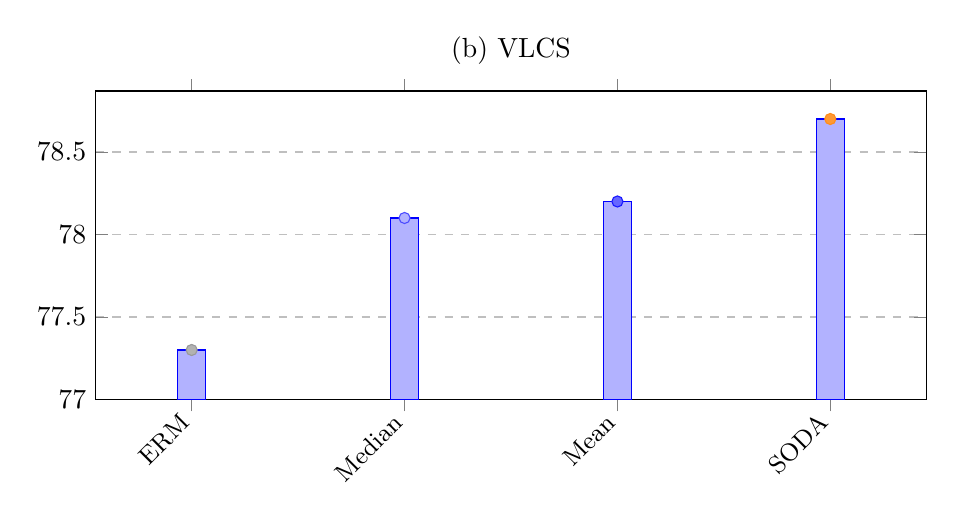
\begin{tikzpicture}
            \begin{axis}[stats multiplot style, title={(b) VLCS}, ymin=77]
                \addplot+[scatter, scatter src=explicit symbolic] 
                table [meta=class, col sep=comma] {
                    x,      y,      class
                    ERM,    77.3,   ERM_class
                    Median, 78.1,   median_class
                    Mean,   78.2,   mean_class
                    SODA,   78.7,   soda_class
                };
            \end{axis}
        \end{tikzpicture}
    \end{subfigure}
    \hfill
    \begin{subfigure}{0.32\textwidth}
        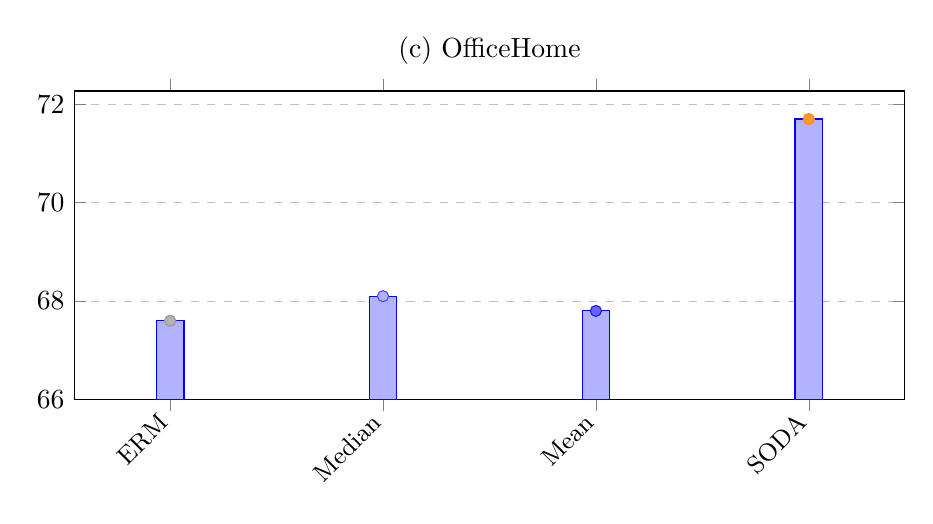
\begin{tikzpicture}
            \begin{axis}[stats multiplot style, title={(c) OfficeHome}, ymin=66]
                \addplot+[scatter, scatter src=explicit symbolic] 
                table [meta=class, col sep=comma] {
                    x,      y,      class
                    ERM,    67.6,   ERM_class
                    Median, 68.1,   median_class
                    Mean,   67.8,   mean_class
                    SODA,   71.7,   soda_class
                };
            \end{axis}
        \end{tikzpicture}
    \end{subfigure}

    \vspace{0.5cm}

    \begin{subfigure}{0.32\textwidth}
        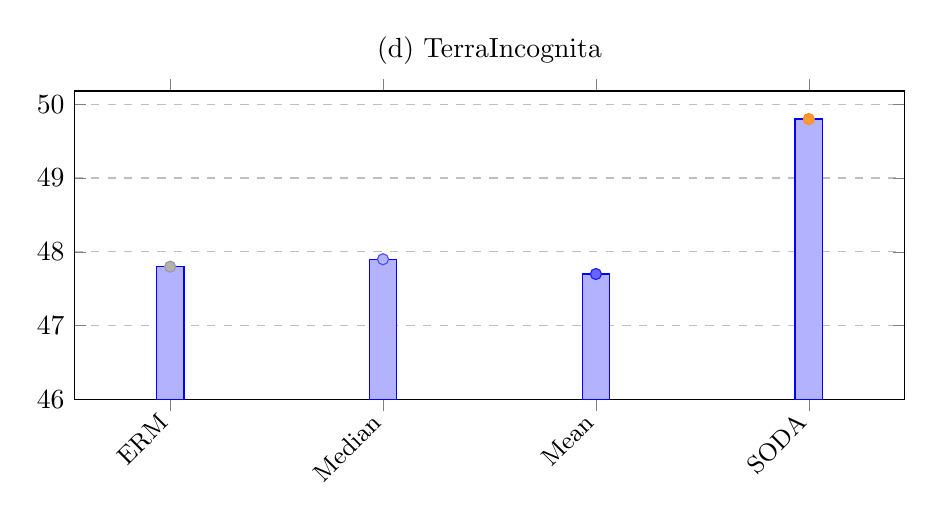
\begin{tikzpicture}
            \begin{axis}[stats multiplot style, title={(d) TerraIncognita}, ymin=46]
                \addplot+[scatter, scatter src=explicit symbolic] 
                table [meta=class, col sep=comma] {
                    x,      y,      class
                    ERM,    47.8,   ERM_class
                    Median, 47.9,   median_class
                    Mean,   47.7,   mean_class
                    SODA,   49.8,   soda_class
                };
            \end{axis}
        \end{tikzpicture}
    \end{subfigure}
    \hfill
    \begin{subfigure}{0.32\textwidth}
        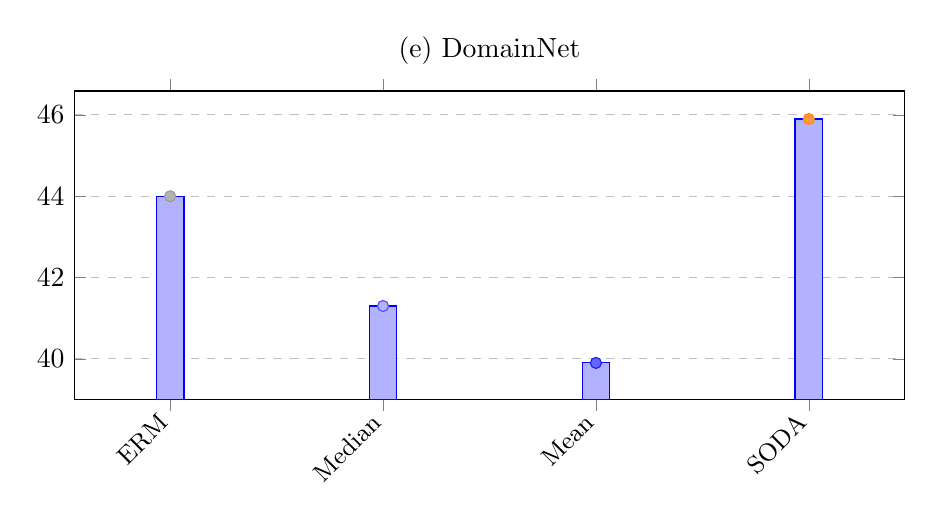
\begin{tikzpicture}
            \begin{axis}[stats multiplot style, title={(e) DomainNet}, ymin=39]
                \addplot+[scatter, scatter src=explicit symbolic] 
                table [meta=class, col sep=comma] {
                    x,      y,      class
                    ERM,    44.0,   ERM_class
                    Median, 41.3,   median_class
                    Mean,   39.9,   mean_class
                    SODA,   45.9,   soda_class
                };
            \end{axis}
        \end{tikzpicture}
    \end{subfigure}
    \hfill
    \begin{subfigure}{0.32\textwidth}
        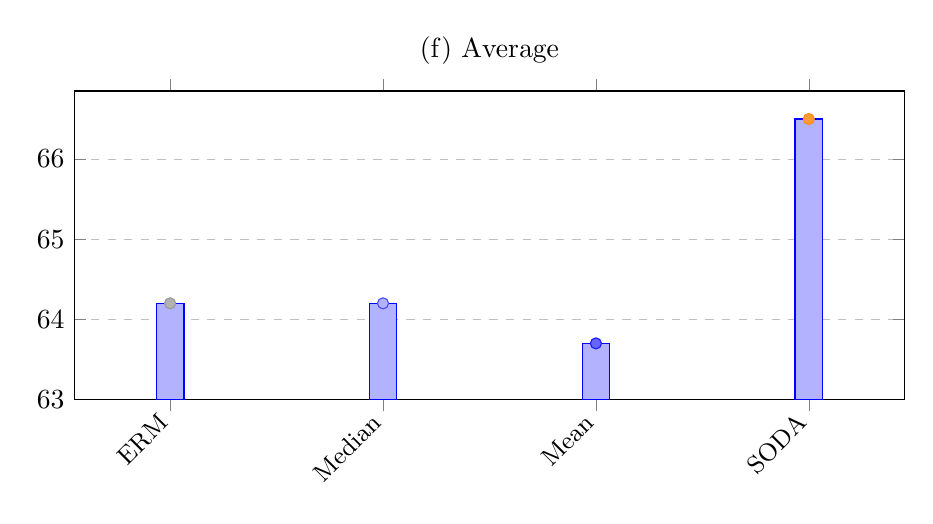
\begin{tikzpicture}
            \begin{axis}[stats multiplot style, title={(f) Average}, ymin=63]
                \addplot+[scatter, scatter src=explicit symbolic] 
                table [meta=class, col sep=comma] {
                    x,      y,      class
                    ERM,    64.2,   ERM_class
                    Median, 64.2,   median_class
                    Mean,   63.7,   mean_class
                    SODA,   66.5,   soda_class
                };
            \end{axis}
        \end{tikzpicture}
    \end{subfigure}

    \caption{Performance of SODA compared against the ERM baseline and the statistical distribution (Mean, Median) of eight state-of-the-art methods across all benchmarks. 
    The figure highlights SODA's robust performance; it consistently surpasses the average and median baseline accuracy. On key challenging datasets like OfficeHome and on the overall Average, it achieves a new state-of-the-art, demonstrating the effectiveness of the stabilized alignment strategy.}
    \label{fig:all_results_stats}
\end{figure*}
We conduct extensive experiments to evaluate SODA across diverse domain generalization scenarios. Our evaluation addresses four key questions:
\begin{enumerate}
    \item How does SODA compare against state-of-the-art domain generalization methods?
    \item What is the contribution of the Dynamic Feature Reservoir to stable alignment?
    \item Can we quantitatively measure the stability improvement provided by SODA?
    \item What are the limitations and failure cases of our approach?
\end{enumerate}

\subsection{Experimental Setup}
\label{ssec:setup}

\subsubsection{Datasets}

We evaluate on seven benchmarks chosen to test different aspects of generalization, summarized in Table~\ref{tab:datasets}.

\begin{table}[t]
\caption{Dataset statistics. Datasets span synthetic controlled environments and real-world vision tasks with diverse domain shift types.}
\label{tab:datasets}
\centering
\small
\begin{tabular}{lcccl}
\toprule
\textbf{Dataset} & \textbf{Domains} & \textbf{Classes} & \textbf{Samples} & \textbf{Shift Type} \\
\midrule
ColoredMNIST & 3 & 2 & 70,000 & Spurious correlation \\
RotatedMNIST & 6 & 10 & 70,000 & Geometric transform \\
PACS & 4 & 7 & 9,991 & Artistic style \\
VLCS & 4 & 5 & 10,729 & Camera/dataset \\
OfficeHome & 4 & 65 & 15,588 & Visual domain \\
TerraIncognita & 4 & 10 & 24,788 & Location/environment \\
DomainNet & 6 & 345 & 586,575 & Large-scale style \\
\bottomrule
\end{tabular}
\end{table}

\textbf{Synthetic Benchmarks.} ColoredMNIST~\citep{arjovsky2019invariant} tests robustness against spurious correlations by associating digit color with labels in training domains but reversing this correlation at test time. RotatedMNIST~\citep{ghifary2015domain} evaluates geometric invariance by rotating digits at different angles across domains.

\textbf{Real-World Benchmarks.} PACS~\citep{li2017deeper} contains images across Photo, Art, Cartoon, and Sketch styles, testing artistic style invariance. VLCS~\citep{fang2013unbiased} aggregates images from four different datasets (PASCAL VOC, LabelMe, Caltech, Sun), representing camera and dataset bias. OfficeHome~\citep{venkateswara2017deep} features 65 object categories across Art, Clipart, Product, and Real-World domains, providing fine-grained domain shift evaluation. TerraIncognita~\citep{beery2018recognition} contains wildlife camera trap images from four geographic locations, representing location-conditioned environmental shift. DomainNet~\citep{peng2019moment} is the largest DG benchmark with 345 categories across six visual styles, testing scalability.

The diversity of these benchmarks ensures comprehensive evaluation: ColoredMNIST tests causal feature learning, PACS/OfficeHome test style invariance, VLCS tests dataset bias, TerraIncognita tests environmental factors, and DomainNet tests scalability.

\subsubsection{Evaluation Protocol}

All experiments follow the DomainBed benchmark suite~\citep{gulrajani2020search} to ensure fair and reproducible comparison. We use the leave-one-domain-out protocol: for a dataset with $N$ domains, we train on $N-1$ domains and evaluate on the held-out domain, repeating for each domain as target. This protocol assesses true generalization to unseen distributions.

Model selection uses the training-domain validation strategy prescribed by DomainBed, which reserves 20\% of training data for validation without any access to test domain information. This prevents information leakage that could inflate reported performance. All accuracies are averaged over three independent runs with different random seeds (0, 1, 2) to ensure statistical robustness.

\subsubsection{Implementation Details}

\textbf{Architecture.} We use a ResNet-50 backbone~\citep{he2016deep} pretrained on ImageNet for real-world datasets and a smaller ConvNet for synthetic benchmarks, following DomainBed conventions. Features for OT alignment are extracted from the final average pooling layer ($d' = 2048$ for ResNet-50), representing high-level semantic embeddings.

\textbf{Optimization.} We train using the Adam optimizer~\citep{kingma2014adam} with hyperparameters sampled via random search (60 configurations per experiment) from the space in Table~\ref{tab:hparams}. Training runs for 5,000 steps with batch size 32. The learning rate follows the sampled initial value without scheduling.
\begin{sloppypar} 
\textbf{SODA-Specific Configuration.} The DFR is initialized with L2-normalized random Gaussian vectors and populated with actual features during training. The reservoir is filled with extracted features after $\lceil K/B\rceil=6$ steps (96 features per step); until then part of the pivot consists of the random initial vectors. Sinkhorn is solved with GeomLoss' $\epsilon$-scaling, which performs $L=7$ updates at $\epsilon=0.01$.
\end{sloppypar} 
\textbf{Software and Hardware.} Our implementation uses PyTorch 2.0.1 with Python 3.9. For efficient Sinkhorn computation, we use the \texttt{geomloss} library (v0.2.6)~\citep{feydy2019interpolating}, which provides numerically stable, log-domain GPU implementations. Experiments were conducted on NVIDIA A100 GPUs (40GB) with CUDA 11.8.

\textbf{Reproducibility.} To facilitate reproducibility, we fix random seeds for network initialization, data sampling, and DFR population. Our implementation code and trained model checkpoints will be made publicly available upon publication.

\begin{table}[t]
\caption{Hyperparameter search space. Model selection samples 60 configurations randomly from this space for each experiment.}
\label{tab:hparams}
\centering
\small
\renewcommand{\arraystretch}{1.1}
\begin{tabular}{lc}
\toprule
\multicolumn{2}{c}{\textbf{General Hyperparameters}} \\
\midrule
Learning Rate & $10^{\text{Uniform}(-5, -3.5)}$ \\
Weight Decay & $10^{\text{Uniform}(-6, -2)}$ \\
ResNet Dropout & $\{0.0, 0.1, 0.5\}$ \\
Batch Size & $32$ (fixed) \\
Training Steps & $5000$ (fixed) \\
\midrule
\multicolumn{2}{c}{\textbf{SODA-Specific Hyperparameters}} \\
\midrule
Alignment Weight $\lambda$ & $\{10^{-4}, 10^{-3}, 10^{-2}, 10^{-1}, 1.0\}$ \\
OT Regularization $\epsilon$ & $\{0.01, 0.05, 0.1, 0.5, 1.0\}$ \\
DFR Capacity $K$ & $\{128, 256, 512\}$ \\
\bottomrule
\end{tabular}
\end{table}

\subsubsection{Computational Cost}
\label{sssec:computational_cost}

Table~\ref{tab:timing} compares SODA's computational overhead against the ERM baseline on OfficeHome with ResNet-50 backbone.

\begin{table}[t]
\caption{Computational cost comparison on OfficeHome (ResNet-50, 32 images per source domain, NVIDIA L40S GPU). Total training is the wall-clock time of a 5,000-step run including periodic evaluation.}
\label{tab:timing}
\centering
\small
\begin{tabular}{lccc}
\toprule
\textbf{Method} & \textbf{Time/Step} & \textbf{GPU Memory} & \textbf{Total Training} \\
\midrule
ERM & 0.181s & 8.14 GB & 17.2 min \\
SODA & 0.193s & 8.15 GB & 18.1 min \\
\midrule
\textbf{Overhead} & +7\% & +0.1\% & +5\% \\
\bottomrule
\end{tabular}
\end{table}

The alignment term adds 7\% per training step and a negligible amount of memory, consistent with the 4MB DFR storage and Table~\ref{tab:scalability}. Importantly, SODA incurs zero overhead at inference, as the DFR is discarded after training. The total training time of about 18 minutes per OfficeHome run is practical for standard GPU hardware, making SODA a viable drop-in regularization method.

\subsubsection{Baselines}
\begin{sloppypar} 
We benchmark SODA against 27 state-of-the-art methods spanning major DG paradigms. As a baseline, we use the standard \textbf{Empirical Risk Minimization} (ERM)~\citep{vapnik1999nature}. For invariance learning and robustness, we compare against \textbf{invariance-based} methods including IRM~\citep{arjovsky2019invariant}, VREx~\citep{krueger2021out}, and EQRM~\citep{eastwood2022probable}, as well as the \textbf{distributionally robust} GroupDRO~\citep{sagawa2019distributionally}. We also evaluate strategies based on \textbf{data augmentation}, such as Mixup~\citep{zhang2018mixup}, and \textbf{meta-learning}, including MLDG~\citep{li2018learning_meta} and MTL~\citep{blanchard2021domain}. Given our focus on feature geometry, we provide extensive comparisons with \textbf{domain alignment} methods (CORAL~\citep{sun2016deep}, MMD~\citep{li2018domain_mmd}, DANN~\citep{ganin2016domain}, CDANN~\citep{li2018deep_cdann}) and \textbf{representation learning} approaches (SagNet~\citep{nam2021reducing}, mDSDI~\citep{bui2021exploiting}, RSC~\citep{huang2020self}, ARM~\citep{zhang2021adaptive}). Furthermore, we compare against \textbf{gradient-based} and \textbf{optimization-based} regularization techniques, including Fish~\citep{shi2022gradient}, Fishr~\citep{rame2022fishr}, SAND~\citep{shahtalebi2021sandmask}, AND~\citep{park2021andmask}, as well as SAM~\citep{foret2021sharpness}, GSAM~\citep{zhuang2022surrogate}, and SAGM~\citep{wang2023sharpness}. Finally, we compare against \textbf{recent methods (2024-2025)} such as MIRO~\citep{cha2022domain}, MADG~\citep{madg2023}, DDN~\citep{zhang2023aggregation}, Arith~\citep{Wang2025BalancedDF}, and GGA~\citep{gga2025}. All baseline results are obtained from DomainBed or the respective papers using identical evaluation protocols.
\end{sloppypar} 
\subsection{Main Results}
\label{ssec:main_results}

\subsubsection{Real-World Benchmarks}

Table~\ref{tab:real_results} presents comprehensive comparison on five real-world benchmarks. SODA achieves the highest average accuracy (66.5\%) across all methods, demonstrating consistent cross-benchmark generalization. A comprehensive visual summary is shown in Figure \ref{fig:all_results_stats}.

\begin{table*}[t]
\caption{
    Comprehensive comparison with state-of-the-art methods on five real-world DG benchmarks using a ResNet-50 backbone. 
    Average accuracy (\%) with standard error is reported. 
    The dataset abbreviations correspond to \textbf{OH}: OfficeHome, \textbf{TI}: TerraIncognita, and \textbf{DN}: DomainNet.
    Best accuracies are highlighted in \textbf{bold}.}
\label{tab:real_results}
\centering
\begingroup % Start a group to keep changes local
\footnotesize % Use a smaller font size
% \setlength{\tabcolsep}{4pt} % Reduce space between columns (default is 6pt)
\renewcommand{\arraystretch}{0.4} % You had 0.55, this is a bit more readable
\begin{tabular}{lcccccc}
\toprule
\textbf{Model} & \textbf{PACS} & \textbf{VLCS} & \textbf{OH} & \textbf{TI} & \textbf{DN} & \textbf{Avg} \\
\midrule
ERM \citep{vapnik1999nature} & $84.2 \pm 0.1$ & $77.3 \pm 0.1$ & $67.6 \pm 0.2$ & $47.8 \pm 0.6$ & $44.0 \pm 0.1$ & 64.2 \\
IRM \citep{arjovsky2019invariant} & $83.5 \pm 0.8$ & $78.5 \pm 0.5$ & $64.3 \pm 2.2$ & $47.6 \pm 0.8$ & $33.9 \pm 2.8$ & 61.6 \\
GDRO \citep{sagawa2019distributionally} & $84.4 \pm 0.8$ & $76.7 \pm 0.6$ & $66.0 \pm 0.7$ & $43.2 \pm 1.1$ & $33.3 \pm 0.2$ & 60.7 \\
Mixup \citep{zhang2018mixup} & $84.6 \pm 0.6$ & $77.4 \pm 0.6$ & $68.1 \pm 0.3$ & $47.9 \pm 0.8$ & $39.2 \pm 0.1$ & 63.4 \\
MLDG \citep{li2018learning_meta} & $84.9 \pm 1.0$ & $77.2 \pm 0.4$ & $66.8 \pm 0.6$ & $47.7 \pm 0.9$ & $41.2 \pm 0.1$ & 63.6 \\
CORAL \citep{sun2016deep} & $86.2 \pm 0.3$ & $78.8 \pm 0.6$ & $68.7 \pm 0.3$ & $47.6 \pm 1.0$ & $41.5 \pm 0.1$ & 64.5 \\
MMD \citep{li2018domain_mmd} & $84.7 \pm 0.5$ & $77.5 \pm 0.9$ & $66.3 \pm 0.1$ & $42.2 \pm 1.6$ & $23.4 \pm 9.5$ & 58.8 \\
DANN \citep{ganin2016domain} & $83.6 \pm 0.4$ & $78.6 \pm 0.4$ & $65.9 \pm 0.6$ & $46.7 \pm 0.5$ & $38.3 \pm 0.1$ & 62.6 \\
CDANN \citep{li2018deep_cdann} & $82.6 \pm 0.9$ & $77.5 \pm 0.1$ & $65.8 \pm 1.3$ & $45.8 \pm 1.6$ & $38.3 \pm 0.3$ & 62.0 \\
MTL \citep{blanchard2021domain} & $84.6 \pm 0.5$ & $77.2 \pm 0.4$ & $66.4 \pm 0.5$ & $45.6 \pm 1.2$ & $40.6 \pm 0.1$ & 62.9 \\
SagNet \citep{nam2021reducing} & $86.3 \pm 0.2$ & $77.8 \pm 0.5$ & $68.1 \pm 0.1$ & $48.6 \pm 1.0$ & $40.3 \pm 0.1$ & 64.2 \\
RSC \citep{huang2020self} & $85.2 \pm 0.9$ & $77.1 \pm 0.5$ & $65.5 \pm 0.9$ & $46.6 \pm 1.0$ & $38.9 \pm 0.5$ & 62.7 \\
mDSDI \citep{bui2021exploiting} & $86.2 \pm 0.2$ & $79.0 \pm 0.3$ & $69.2 \pm 0.4$ & $48.1 \pm 1.4$ & $42.8 \pm 0.1$ & 65.1 \\
Fish \citep{shi2022gradient} & $85.5 \pm 0.3$ & $77.8 \pm 0.3$ & $68.6 \pm 0.4$ & $45.1 \pm 1.3$ & $42.7 \pm 0.2$ & 63.9 \\
Fishr \citep{rame2022fishr} & $86.2 \pm 0.2$ & $78.2 \pm 0.2$ & $68.2 \pm 0.2$ & $53.6 \pm 0.4$ & $41.8 \pm 0.2$ & 65.6 \\
SAND \citep{shahtalebi2021sandmask} & $85.2 \pm 0.5$ & $76.2 \pm 0.5$ & $65.9 \pm 0.5$ & $50.2 \pm 0.1$ & $32.2 \pm 0.6$ & 61.9 \\
AND \citep{park2021andmask} & $84.4 \pm 0.4$ & $76.4 \pm 0.4$ & $66.1 \pm 0.2$ & $49.8 \pm 0.4$ & $37.9 \pm 0.6$ & 62.9 \\
MIRO \citep{cha2022domain} & $85.4 \pm 0.4$ & $79.0 \pm 0.0$ & $70.5 \pm 0.4$ & $50.4 \pm 1.1$ & $44.3 \pm 0.2$ & 65.9 \\
% SWAD \citep{cha2021swad} & $88.2 \pm 0.1$ & $79.1 \pm 0.1$ & $70.6 \pm 0.2$ & $50.0 \pm 0.3$ & $46.5 \pm 0.1$ & 66.9 \\
% Stylized \citep{heo2023domain} & $89.0 \pm 0.3$ & $78.8 \pm 0.1$ & $70.4 \pm 0.3$ & $51.1 \pm 1.2$ & $46.4 \pm 0.7$ & 67.2 \\
SAM \citep{foret2021sharpness} & $85.8 \pm 0.2$ & $79.4 \pm 0.1$ & $69.6 \pm 0.1$ & $43.3 \pm 0.7$ & $44.3 \pm 0.0$ & 64.5 \\
GSAM \citep{zhuang2022surrogate} & $85.9 \pm 0.1$ & $79.1 \pm 0.2$ & $69.3 \pm 0.0$ & $47.0 \pm 0.8$ & $44.6 \pm 0.2$ & 65.1 \\
EQRM \citep{eastwood2022probable} & $86.5 \pm 0.2$ & 77.8 $\pm 0.6$ & $67.5 \pm 0.1$ & $47.8 \pm 0.6$ & $41.0 \pm 0.3$ & 64.1 \\
SAGM \citep{wang2023sharpness} & $86.6 \pm 0.2$ & $80.0 \pm 0.3$ & $70.1 \pm 0.2$ & $48.8 \pm 0.9$ & $45.0 \pm 0.2$ & 66.1 \\
MADG \citep{madg2023} & $86.5 \pm 0.4$ & $78.7 \pm 0.2$ & $71.3 \pm 0.3$ & \textbf{53.7} $\pm 0.5$ & $39.9 \pm 0.4$ & 66.0 \\
DDN \citep{zhang2023aggregation} & $87.2 \pm 0.2$ & \textbf{80.3} $\pm 0.2$ & $69.5 \pm 0.2$ & $50.4 \pm 0.5$ & $43.4 \pm 0.1$ & 66.2 \\
Arith \citep{Wang2025BalancedDF} & 86.5 $\pm 0.3$ & 79.4 $\pm 0.3$ & $69.4 \pm 0.1$ & $48.1 \pm 1.2$ & $41.5 \pm 0.1$ & 65.0 \\
GGA \citep{gga2025} & \textbf{87.3} $\pm 0.4$ & 79.9 $\pm 0.4$ & $68.5 \pm 0.2$ & $50.6 \pm 0.1$ & $45.2 \pm 0.2$ & 66.3 \\
\midrule
\textbf{SODA} & $86.5 \pm 0.2$ & $78.7 \pm 0.2$ & \textbf{71.7} $\pm 0.1$ & $49.8 \pm 0.3$ & \textbf{45.9} $\pm 0.3$ & \textbf{66.5} \\
\bottomrule
\end{tabular}
\endgroup % End the group
\end{table*}

\textbf{Key Observations.} SODA achieves state-of-the-art results on OfficeHome (71.7\%) and DomainNet (45.9\%), the two largest and most diverse benchmarks. On the average metric, SODA (66.5\%) outperforms all methods including recent optimization-based approaches like GGA (66.3\%) and DDN (66.2\%). Notably, SODA is the only method achieving above-average performance on all five benchmarks simultaneously, demonstrating consistent generalization rather than dataset-specific optimization.

\textbf{Comparison with Alignment Methods.} Among domain alignment methods (CORAL, MMD, DANN), SODA shows substantial improvements (+2.0\% over CORAL on average), validating that stable OT alignment is more effective than statistical discrepancy minimization or adversarial training.

\textbf{Comparison with Optimization-Based Methods.} Methods like SAM, GSAM, and SAGM regularize the loss landscape geometry, while SODA regularizes the feature space geometry. SODA's competitive performance suggests these approaches are complementary; combining stable alignment with flat minima seeking could yield further gains.

\subsubsection{Synthetic Benchmarks}

Table~\ref{tab:synthetic_results} presents results on controlled synthetic benchmarks that isolate specific generalization challenges.

\begin{table}[t]
\caption{Comparison on synthetic DG benchmarks. Average accuracy (\%) with standard error using training-domain validation. CMNIST: ColoredMNIST, RMNIST: RotatedMNIST.}
\label{tab:synthetic_results}
\centering
\small
\renewcommand{\arraystretch}{1.1}
\begin{tabular}{lcc}
\toprule
\textbf{Algorithm} & \textbf{CMNIST} & \textbf{RMNIST} \\
\midrule
ERM \citep{vapnik1999nature} & $51.5 \pm 0.1$ & $98.0 \pm 0.0$ \\
IRM \citep{arjovsky2019invariant} & $52.0 \pm 0.1$ & $97.7 \pm 0.1$ \\
GroupDRO \citep{sagawa2019distributionally} & $52.1 \pm 0.0$ & $98.0 \pm 0.0$ \\
Mixup \citep{yan2020improve} & $52.1 \pm 0.2$ & $98.0 \pm 0.1$ \\
MLDG \citep{li2018learning_meta} & $51.5 \pm 0.1$ & $97.9 \pm 0.0$ \\
CORAL \citep{sun2016deep} & $51.5 \pm 0.1$ & $98.0 \pm 0.1$ \\
MMD \citep{li2018domain_mmd} & $51.5 \pm 0.2$ & $97.9 \pm 0.0$ \\
DANN \citep{ganin2016domain} & $51.5 \pm 0.3$ & $97.8 \pm 0.1$ \\
CDANN \citep{li2018deep_cdann} & $51.7 \pm 0.1$ & $97.5 \pm 0.1$ \\
MTL \citep{blanchard2021domain} & $51.4 \pm 0.1$ & $97.9 \pm 0.0$ \\
SagNet \citep{nam2021reducing} & $51.7 \pm 0.0$ & $98.0 \pm 0.0$ \\
ARM \citep{zhang2021adaptive} & $56.2 \pm 0.2$ & $98.2 \pm 0.1$ \\
VREx \citep{krueger2021out} & $51.8 \pm 0.1$ & $97.9 \pm 0.1$ \\
RSC \citep{huang2020self} & $51.7 \pm 0.2$ & $97.6 \pm 0.1$ \\
\midrule
\textbf{SODA (Ours)} & \textbf{58.1} $\pm 0.1$ & \textbf{98.3} $\pm 0.1$ \\
\bottomrule
\end{tabular}
\end{table}

On ColoredMNIST, SODA achieves 58.1\%, substantially outperforming ERM (51.5\%) and other methods. This benchmark specifically tests robustness against spurious correlations where color is predictive in training domains but anti-correlated at test time. The strong improvement indicates that stable geometric alignment helps the model learn the true invariant features (digit shape) rather than domain-specific shortcuts (color). On RotatedMNIST, SODA achieves 98.3\%, demonstrating effective learning of rotational invariance.

\subsection{Ablation Studies}
\label{ssec:ablation}

We conduct detailed ablation studies on OfficeHome due to its significant domain variety and sensitivity to alignment strategy choices.

\subsubsection{Effect of Pivot Strategy}

Table~\ref{tab:ablation_pivot} isolates the contribution of the DFR by comparing against alternative pivot strategies.

\begin{table}[t]
\caption{Effect of alignment strategy on OfficeHome. Results quantify the benefit of the DFR pivot over batch-derived and alternative targets.}
\label{tab:ablation_pivot}
\centering
\small
\renewcommand{\arraystretch}{1.1}
\begin{tabular}{lcc}
\toprule
\textbf{Strategy} & \textbf{Accuracy (\%)} & \textbf{Std. Error} \\
\midrule
ERM (No Alignment) & 67.6 & $\pm 0.2$ \\
\midrule
\multicolumn{3}{l}{\textit{Batch-Derived Pivots:}} \\
\quad Pooled-Target OT & 67.8 & $\pm 0.3$ \\
\quad Standard Pivot OT & 71.0 & $\pm 0.2$ \\
\midrule
\multicolumn{3}{l}{\textit{Advanced Alternatives:}} \\
\quad Pairwise OT & 70.6 & $\pm 0.2$ \\
\quad Gromov-Wasserstein OT & 70.9 & $\pm 0.3$ \\
\midrule
\textbf{SODA (DFR Pivot)} & \textbf{71.7} & $\pm 0.1$ \\
\bottomrule
\end{tabular}
\end{table}

\textbf{Analysis.} ERM (67.6\%) provides the baseline without alignment. Pooled-Target OT, which uses the minibatch feature centroid as pivot, achieves only 67.8\%, demonstrating that unstable pivots provide negligible benefit. Standard Pivot OT (randomly selected source domain as pivot) reaches 71.0\%, showing that even noisy but structured pivots help. Pairwise OT (70.6\%) and Gromov-Wasserstein OT (70.9\%), despite their theoretical appeal, are hampered by batch-derived target variance.

SODA (71.7\%) achieves the best performance by providing a stable, high-capacity pivot. The lower standard error ($\pm 0.1$ vs. $\pm 0.3$ over three runs) is consistent with more stable optimization, which Section~\ref{ssec:stability_analysis} examines through the variance of the alignment gradient.

\textbf{Class-conditional reservoir.} Because the ground cost ignores labels, a source feature may be transported toward reservoir features of other classes. We therefore evaluate a class-conditional variant that keeps the same FIFO reservoir but assigns a prohibitive cost ($\beta/\epsilon=50$) to pairs with different labels and reweights the reservoir marginal to the class histogram of the source batch, so that the loss becomes $\sum_c \hat p_c W_\epsilon(\alpha_c,\beta_c)$ over the classes present in both. Separate per-class queues would hold only about eight entries per class on OfficeHome with $K=512$. Over the same three seeds, the class-conditional variant reaches 70.9\% against 70.8\% for the class-agnostic DFR. The transport plans explain why: in the class-agnostic plan, the fraction of mass sent between different classes is $0.61$--$0.62$, close to the minimum $0.60$--$0.61$ that any plan must move because the class histograms of a 32-sample batch and of the reservoir differ, and far from the $0.98$ of an independent coupling. Only about 1\% of the mass crosses classes beyond this minimum.

\subsubsection{Effect of DFR Capacity}

Table~\ref{tab:ablation_dfr_k} examines how reservoir capacity $K$ affects performance.

\begin{table}[t]
\caption{Effect of DFR capacity $K$ on OfficeHome. Per-domain accuracy (\%) reported for Art (A), Clipart (C), Product (P), and Real-World (R) as target domains.}
\label{tab:ablation_dfr_k}
\centering
\small
\renewcommand{\arraystretch}{1.1}
\begin{tabular}{ccccc|c}
\toprule
\textbf{$K$} & \textbf{A} & \textbf{C} & \textbf{P} & \textbf{R} & \textbf{Avg} \\
\midrule
128 & 55.6 & 78.7 & 67.0 & 81.2 & 70.6 \\
256 & 56.4 & 80.2 & 67.0 & 81.3 & 71.2 \\
512 & 57.7 & 78.8 & 66.6 & 81.9 & 71.3 \\
\bottomrule
\end{tabular}
\end{table}

\textbf{Analysis.} Performance improves monotonically from $K=128$ (70.6\%) to $K=512$ (71.3\%), with the largest gain on the Art domain (+2.1\%). This aligns with our theoretical analysis: the pivot-induced variance of the alignment gradient decreases with $K$ (Table~\ref{tab:gradvar}).

The relationship between $K$ and stability can be understood through our Definition~\ref{def:stability}: with $K=512$ and $B=96$ features per step, 18.75\% of the reservoir changes per iteration, yielding high pivot stability. The diminishing returns from $K=256$ to $K=512$ (+0.1\%) suggest that $K=256$ already provides sufficient stability for this dataset, though $K=512$ offers marginally better performance at negligible memory cost (4MB).

\subsubsection{Sensitivity to OT Hyperparameters}

Table~\ref{tab:ablation_ot} analyzes sensitivity to alignment weight $\lambda$ and regularization strength $\epsilon$.

\begin{table}[t]
\caption{Sensitivity to OT hyperparameters on OfficeHome. Per-domain accuracy (\%) for Art (A), Clipart (C), Product (P), and Real-World (R).}
\label{tab:ablation_ot}
\centering
\small
\renewcommand{\arraystretch}{1.1}
\begin{tabular}{lcccc|c}
\toprule
\textbf{Setting} & \textbf{A} & \textbf{C} & \textbf{P} & \textbf{R} & \textbf{Avg} \\
\midrule
\multicolumn{6}{l}{\textit{Alignment Weight $\lambda$:}} \\
$\lambda = 10^{-4}$ & 57.9 & 79.6 & 66.6 & 80.9 & 71.3 \\
$\lambda = 10^{-3}$ & 56.8 & 80.2 & 66.9 & 81.3 & 71.3 \\
$\lambda = 10^{-2}$ & 57.7 & 78.8 & 67.0 & 81.4 & 71.2 \\
$\lambda = 10^{-1}$ & 56.4 & 79.3 & 66.4 & 81.1 & 70.8 \\
$\lambda = 1.0$ & 55.9 & 80.4 & 68.1 & 81.2 & 71.4 \\
\midrule
\multicolumn{6}{l}{\textit{OT Regularization $\epsilon$:}} \\
$\epsilon = 0.01$ & 56.4 & 79.5 & 66.5 & 81.1 & 70.9 \\
$\epsilon = 0.05$ & 57.6 & 80.1 & 66.9 & 81.4 & 71.5 \\
$\epsilon = 0.1$ & 55.6 & 78.7 & 68.1 & 81.3 & 70.9 \\
$\epsilon = 0.5$ & 58.0 & 79.0 & 66.6 & 80.8 & 71.1 \\
$\epsilon = 1.0$ & 57.9 & 80.4 & 67.0 & 81.0 & 71.6 \\
\bottomrule
\end{tabular}
\end{table}

\textbf{Alignment Weight $\lambda$.} Performance is relatively stable across four orders of magnitude ($10^{-4}$ to $1.0$), ranging from 70.8\% to 71.4\%. This robustness indicates that the DFR's stable pivot provides reliable gradients regardless of the loss weighting, reducing hyperparameter sensitivity.

\textbf{OT Regularization $\epsilon$.} Higher regularization ($\epsilon = 1.0$) yields the best average performance (71.6\%), outperforming lower values that approximate the exact Wasserstein distance more closely. This finding aligns with Proposition~\ref{prop:entropy}: lower $\epsilon$ induces sparse transport plans where gradients concentrate on nearest-neighbor matches, making optimization sensitive to individual reservoir entries. Higher $\epsilon$ produces diffuse plans where each source feature receives gradient contributions from multiple target features, providing geometric regularization against overfitting to specific reservoir samples.

\subsection{Quantitative Stability Analysis}
\label{ssec:stability_analysis}

To directly validate our theoretical claims about pivot stability, we analyze inter-run standard error as a proxy for optimization stability.

\begin{table}[t]
\caption{Stability comparison: inter-run standard error over three runs across methods on OfficeHome.}
\label{tab:stability_comparison}
\centering
\small
\begin{tabular}{lcc}
\toprule
\textbf{Method} & \textbf{Accuracy} & \textbf{Std. Error (3 runs)} \\
\midrule
Pooled-Target OT & 67.8\% & $\pm 0.3$ \\
Gromov-Wasserstein OT & 70.9\% & $\pm 0.3$ \\
Standard Pivot OT & 71.0\% & $\pm 0.2$ \\
Pairwise OT & 70.6\% & $\pm 0.2$ \\
\textbf{SODA (DFR)} & \textbf{71.7\%} & $\pm 0.1$ \\
\bottomrule
\end{tabular}
\end{table}

As shown in Table~\ref{tab:stability_comparison}, methods with batch-derived pivots exhibit higher inter-run standard error ($\pm 0.2$--$0.3$). SODA has the lowest standard error ($\pm 0.1$). With three runs per method this comparison is only indicative, so we also measure the variance of the alignment gradient directly.

\textbf{Gradient variance.} We take SODA checkpoints after 500, 1,000, 2,500 and 5,000 steps, fix 16 source minibatches, and for each of them draw 16 pivots independently of the source batch, which isolates the pivot-induced part of the gradient variance (Section~\ref{ssec:pivot_instability}). Table~\ref{tab:gradvar} reports this variance relative to the squared norm of the mean gradient, both for the gradient with respect to the source features and for the parameters of the last ResNet stage. A reservoir of $K=512$ reduces it by a factor of 4 to 9 in feature space and 6 to 29 in parameter space compared with batch-derived pivots, and the variance decreases roughly as $1/K$. With batch-derived pivots the relative variance exceeds 1, i.e., the variation of the gradient across pivots is larger than its mean.

\begin{table}[t]
\caption{Pivot-induced variance of the alignment gradient relative to the squared norm of the mean gradient, OfficeHome (Art as test domain), 16 source batches $\times$ 16 pivots, $\epsilon=0.01$. Feat.: gradient w.r.t.\ the normalized features; Param.: w.r.t.\ the last ResNet stage.}
\label{tab:gradvar}
\centering
\small
\begin{tabular}{lcccc}
\toprule
 & \multicolumn{2}{c}{step 500} & \multicolumn{2}{c}{step 5000} \\
Pivot & Feat. & Param. & Feat. & Param. \\
\midrule
DFR, $K=128$ & 0.93 & 1.05 & 1.41 & 1.37 \\
DFR, $K=256$ & 0.52 & 0.47 & 0.58 & 0.43 \\
DFR, $K=512$ & 0.28 & 0.24 & 0.19 & 0.15 \\
DFR, $K=1024$ & 0.10 & 0.10 & 0.09 & 0.07 \\
Single source domain (32) & 1.34 & 2.96 & 1.36 & 4.29 \\
Pooled batch (96) & 1.09 & 1.37 & 1.66 & 2.04 \\
\bottomrule
\end{tabular}
\end{table}

This supports our theoretical analysis: by reducing pivot instability $\mathcal{S}$ (Definition~\ref{def:stability}), the DFR reduces the pivot-induced gradient variance (Proposition~\ref{prop:gradient_variance}), leading to more consistent optimization trajectories.

\subsection{Analysis of Performance Variations}
\label{ssec:failure_analysis}

While SODA achieves strong average performance, examining cases where it underperforms provides insight into its mechanisms and limitations.

\subsubsection{TerraIncognita Analysis}

SODA achieves 49.8\% on TerraIncognita, below MADG's 53.7\% and Fishr's 53.6\%. TerraIncognita presents wildlife images from camera traps across four geographic locations (L100, L38, L43, L46), where domain shift manifests through ecosystem appearance and camera viewpoint variations.

We hypothesize two factors contribute to this gap:
\begin{sloppypar} 
\textbf{Location-specific feature importance.} Unlike style-based shifts (PACS, OfficeHome) where global feature statistics capture domain differences, location-based shifts may require preserving discriminative local features. Global distribution alignment may inadvertently smooth location-specific patterns that are actually predictive for wildlife identification.
\end{sloppypar} 
\subsubsection{VLCS Analysis}

SODA (78.7\%) trails DDN (80.3\%) and SAGM (80.0\%) on VLCS. This benchmark aggregates images from four photographic datasets with relatively subtle domain shifts compared to the artistic style variations in PACS.

When domain shifts are mild, explicit distribution alignment may provide diminishing returns compared to methods that directly regularize feature geometry (DDN) or optimize for flat loss landscapes (SAGM). The overhead of computing transport plans may not be justified when simpler statistical alignment suffices.

\subsubsection{Class Imbalance}

The DFR stores features of all classes, so its class histogram follows the class frequencies of recent source batches: a class with frequency $\pi_c$ has on average $K\pi_c$ entries and is absent with probability about $(1-\pi_c)^K$. Rare classes are therefore under-represented in the pivot. To test whether this harms them, we compare the per-class test recall of SODA with that of the same model trained without the alignment term ($\lambda=0$), over 10 seeds, and relate the difference to the class frequency in the source domains. On TerraIncognita, whose class distribution is strongly imbalanced, the change in recall is unrelated to class frequency (Spearman $\rho=0.02$, $p=0.92$) and the rarest 20\% of classes gain as much as the most frequent 20\% ($+0.9$ points each); on PACS and VLCS there is no significant relation either. On OfficeHome the gain is slightly larger for frequent classes (under 1 point), and the class-balanced accuracy of SODA and of the model without alignment differs by less than $0.2$ points on every dataset. Section~\ref{ssec:ablation} additionally evaluates a class-conditional reservoir.

\subsubsection{Consistency Analysis}

Despite underperforming on individual benchmarks, SODA demonstrates the most consistent cross-benchmark performance:

\begin{itemize}
    \item SODA is the only method achieving $\geq 66\%$ average across all methods
    \item No single competitor outperforms SODA on more than two benchmarks
    \item Methods excelling on specific datasets often underperform elsewhere (e.g., MADG: 53.7\% on TI but 39.9\% on DN)
\end{itemize}

This consistency suggests that stable geometric alignment provides a robust foundation for diverse domain shifts, even if specialized methods may excel on particular shift types.

\subsection{Qualitative Analysis}
\label{ssec:visualization}

\begin{figure*}[t]
    \centering
    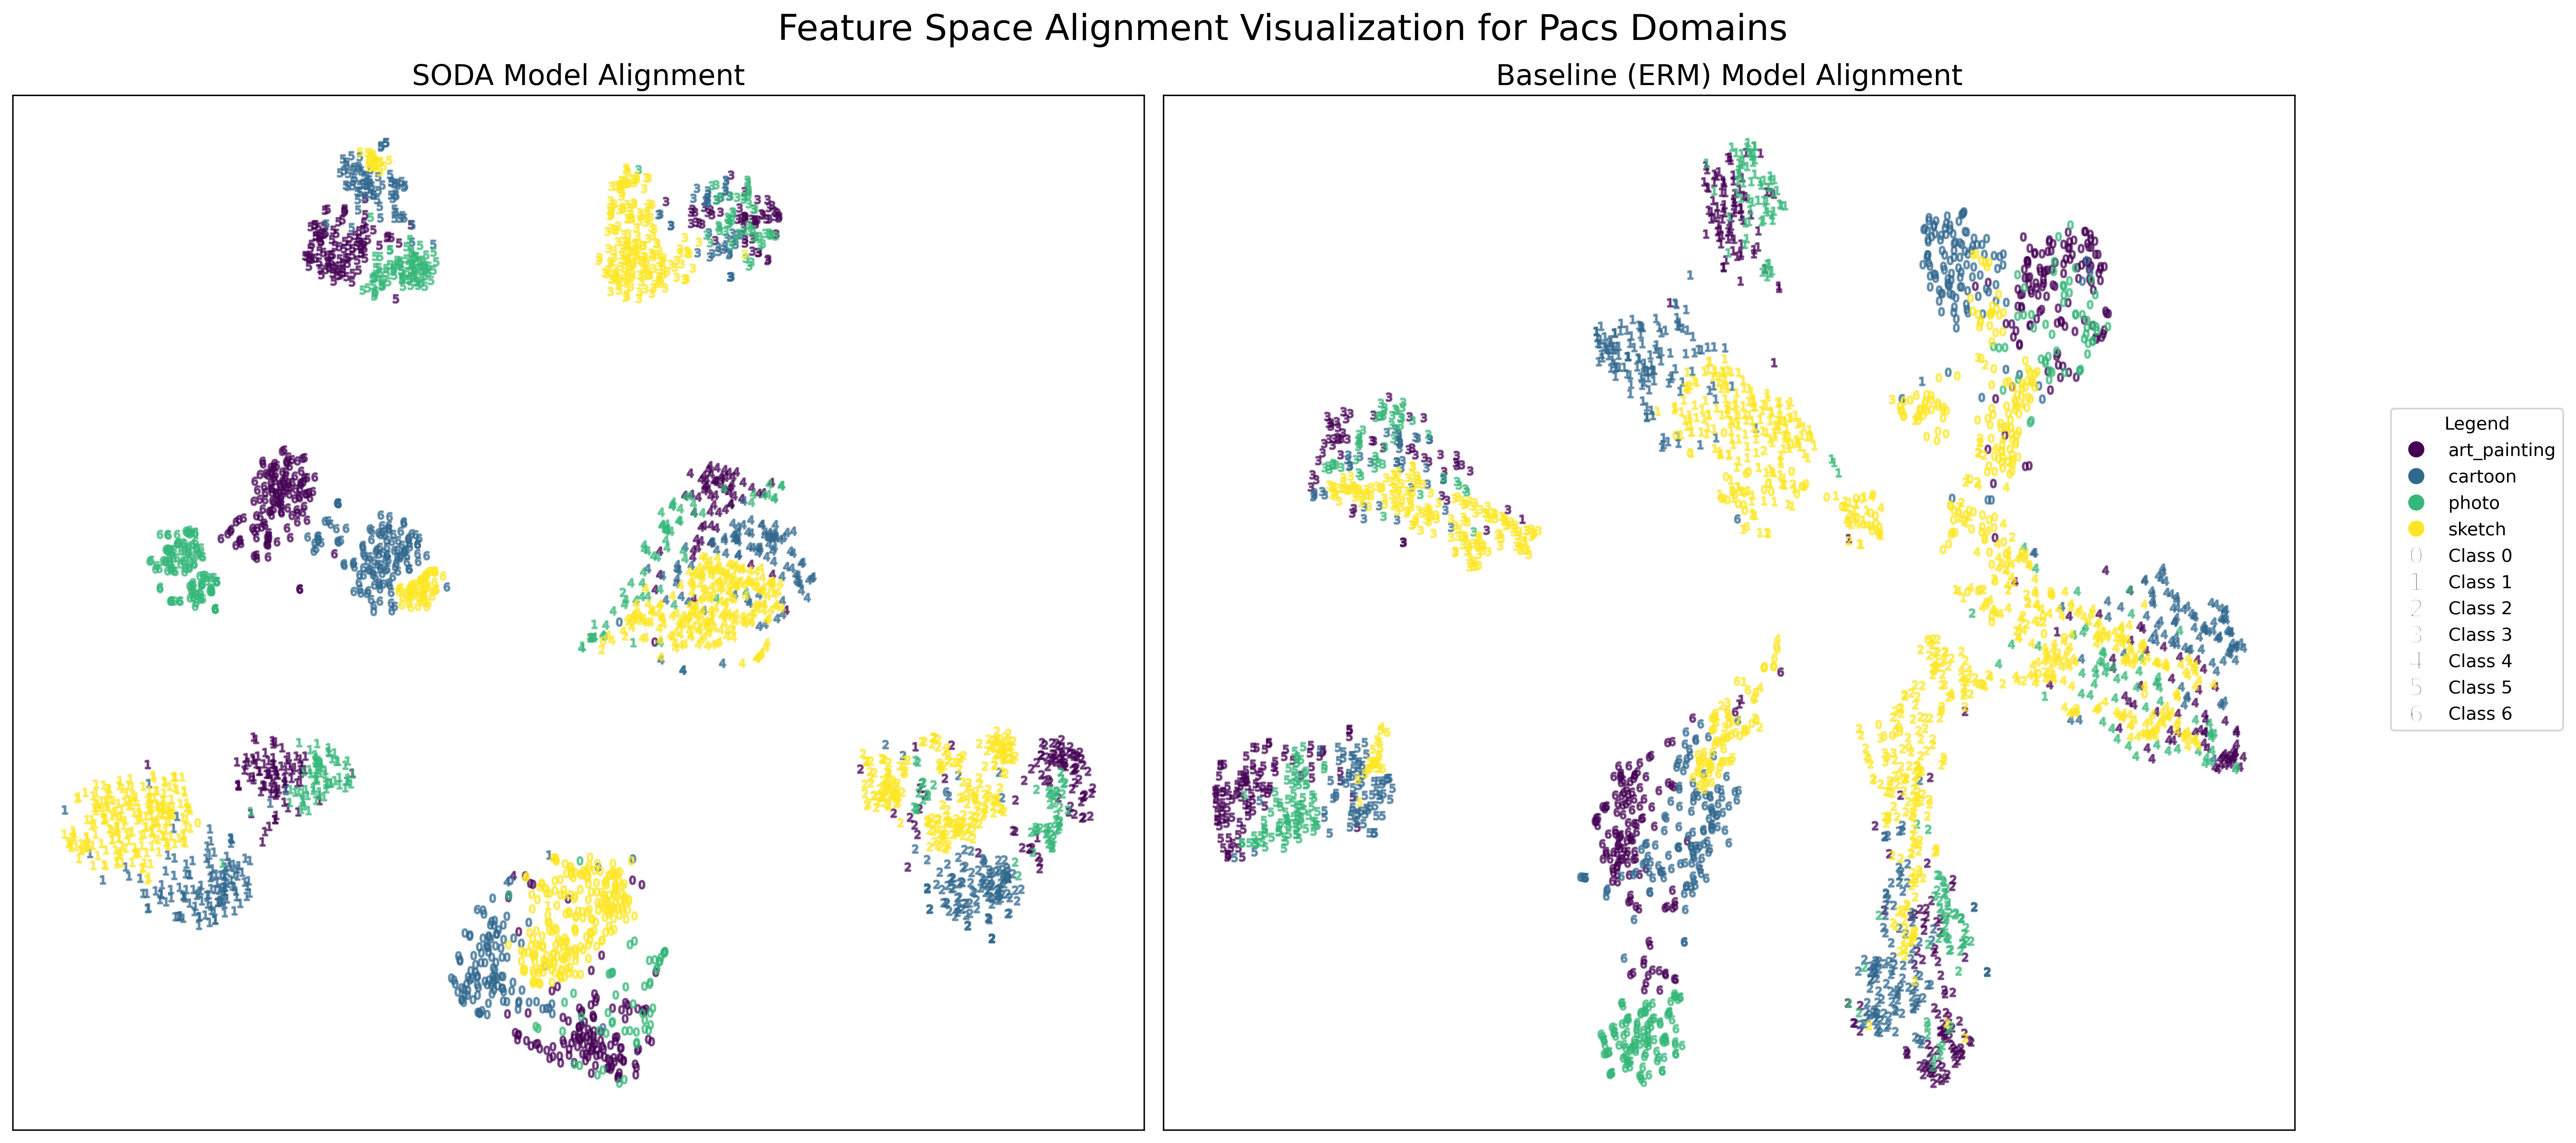
\includegraphics[width=0.95\textwidth]{fig/alignment_pacsClear.png}
    \caption{t-SNE visualization of ResNet-50 features on PACS with Art as target domain. Points are colored by domain and labeled by class. (a) ERM exhibits domain-based clustering, indicating failure to learn invariant features. (b) SODA achieves class-based clustering with domain intermixing, demonstrating successful domain-invariant representation learning.}
    \label{fig:tsne_sota}
\end{figure*}

Figure~\ref{fig:tsne_sota} visualizes the learned feature space using t-SNE~\citep{van2008visualizing} on PACS with Art as the target domain.

\textbf{ERM Baseline (Left).} Features cluster primarily by domain origin rather than semantic class. The Photo, Cartoon, and Sketch domains form distinct clusters, indicating that the model has learned domain-specific features that fail to transfer to the unseen Art domain.

\textbf{SODA (Right).} Domain-based clusters dissolve, and features organize into tight class-based clusters with samples from different domains intermixed. This visualization confirms that SODA successfully learns domain-invariant representations where semantic content, not domain origin, determines feature similarity.

The qualitative improvement aligns with our quantitative results: by providing a stable alignment target, the DFR enables the feature extractor to learn genuinely invariant representations rather than domain-specific artifacts.


\begin{figure}[t]
    \centering
    % Replace 'figure_filename' with the actual name of your image file
    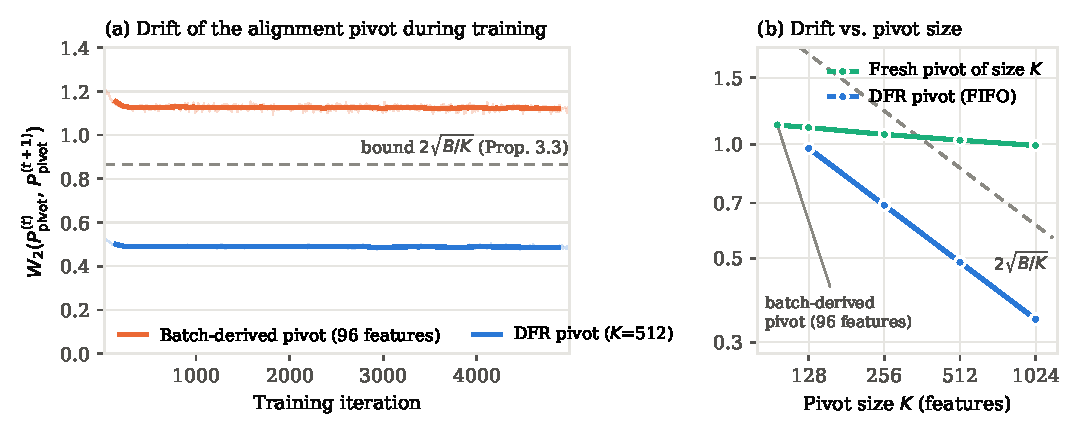
\includegraphics[width=1.0\linewidth]{fig/target_drift_v2.pdf}
    \caption{\textbf{Quantitative Stability Analysis.} Exact Wasserstein-2 distance between the alignment pivots of consecutive training iterations ($W_2(P_{\text{pivot}}^{(t)}, P_{\text{pivot}}^{(t+1)})$), computed from the features logged during a SODA run on OfficeHome. (a) The batch-derived pivot (orange) drifts by about 1.13 throughout training, while the DFR pivot with $K=512$ (blue) drifts by 0.49, below the bound $2\sqrt{B/K}$ of Proposition~\ref{prop:dfr_stability} (dashed). (b) The drift of the DFR follows the $\sqrt{B/K}$ scaling of the bound for every $K$, whereas a freshly drawn pivot of the same size drifts almost as much as the batch pivot: the stability of the DFR comes from the overlap of consecutive reservoirs.}
    \label{fig:stability_analysis}
\end{figure}

\subsection{Stability Analysis}
\label{sec:stability_analysis}

To directly validate our theoretical claims regarding pivot instability and the smoothing effect of the DFR (Proposition~\ref{prop:dfr_stability}), we monitor the temporal evolution of the alignment target. In Figure~\ref{fig:stability_analysis}, we plot the \textbf{Target Drift}, defined as the Wasserstein-2 distance between the pivot distribution used at iteration $t$ and the pivot used at $t+1$.

As shown in Figure~\ref{fig:stability_analysis}(a), a pivot constructed solely from the current mini-batch drifts by $W_2\approx1.13$ between consecutive iterations throughout training. This confirms the impact of the statistical impossibility result~\citep{dong2025distribution}: when the feature dimension ($d'=2048$) far exceeds the batch size ($B=32$), the empirical distribution is dominated by sampling variance rather than the true underlying manifold structure. Consequently, the feature extractor receives noisy, conflicting gradient signals across iterations.

In contrast, the DFR pivot with $K=512$ drifts by $0.49$, 2.3 times less, and stays below the bound $2\sqrt{B/K}=0.87$ of Proposition~\ref{prop:dfr_stability}. Figure~\ref{fig:stability_analysis}(b) shows that this drift follows the $\sqrt{B/K}$ scaling for every $K$, whereas a freshly drawn pivot of the same size drifts almost as much as the batch pivot. The stability therefore comes from the overlap of consecutive reservoirs, which acts as a low-pass filter for the feature distribution, providing the stable geometric anchor necessary for the entropic OT cost to approximate the true domain distance effectively.

\textbf{Staleness.} To quantify the bias of Proposition~\ref{prop:staleness}, we keep the input images of the batches that are still in the reservoir and periodically re-encode them with the current model (every step during the first 300 steps, then every 50 steps), on OfficeHome with each test domain. For the two configurations without dropout, the mean displacement between stored and re-encoded reservoir features is $0.07$ during the first 300 steps and $0.025$ after step 1,000; the resulting change of the alignment loss is $0.003$ and $0.001$, about 50 times below the bound, and the alignment gradients computed with the stored and with the re-encoded reservoir have cosine similarity $0.994$--$0.998$. For the two configurations with dropout $0.5$, the displacement ($0.767$) equals that of the current batch re-encoded without dropout ($0.765$), so staleness adds almost nothing to the noise introduced by dropout. Since no entry is older than $\lceil K/B\rceil=6$ steps, staleness remains small throughout training, including the early phase.



\subsection{Summary of Experimental Findings}

Our experiments validate the following claims:

\begin{enumerate}
    \item \textbf{State-of-the-art performance}: SODA achieves the highest average accuracy (66.5\%) across seven benchmarks, with particular strength on large-scale datasets (OfficeHome, DomainNet).
    
    \item \textbf{Pivot stability matters}: The DFR reduces the pivot-induced variance of the alignment gradient by a factor of 4 to 9 compared to batch-derived pivots.
    
    \item \textbf{Robustness to hyperparameters}: Performance remains stable across wide ranges of $\lambda$ and $\epsilon$, reducing practical tuning burden.
    
    
    \item \textbf{Practical efficiency}: The 7\% per-step training overhead and zero inference cost make SODA a viable drop-in regularization method for standard GPU hardware.
\end{enumerate}